\documentclass[a4paper, 12pt]{article} % Font size (can be 10pt, 11pt or 12pt) and paper size (remove a4paper for US letter paper)
\usepackage[portuguese]{babel}

\usepackage[protrusion=true,expansion=true]{microtype} % Better typography
\usepackage{graphicx} % Required for including pictures
\usepackage{wrapfig} % Allows in-line images
\usepackage{pdflscape} %Allows landscape oriented pages

\usepackage{hyperref}%Required for hyperlink references
\hypersetup{
	colorlinks=true, % Ativa links coloridos em vez de caixas ao redor
	linkcolor=black, % Cor dos links internos
	citecolor=black, % Cor das citações
	urlcolor=black   % Cor dos links externos (Jira, por exemplo)
}

\usepackage{mathpazo} % Use the Palatino font
\usepackage[T1]{fontenc} % Required for accented characters
\linespread{1.05} % Change line spacing here, Palatino benefits from a slight increase by default
\usepackage{float}
\usepackage[backend=bibtex,style=numeric]{biblatex}
\addbibresource{references.bib} % Nome do arquivo de referências
\makeatletter
\renewcommand\@biblabel[1]{\textbf{#1.}} % Change the square brackets for each bibliography item from '[1]' to '1.'
\renewcommand{\@listI}{\itemsep=0pt} % Reduce the space between items in the itemize and enumerate environments and the bibliography

\renewcommand{\maketitle}{
\begin{titlepage}
\begin{center}
\vspace*{1cm}
% \includegraphics[width=0.35\textwidth]{../images/logo-no-bg.png}\\[1cm] % Logo
{\Huge\textbf{Trabalho Prático 1}}\\[0.5cm] % Main Title
{\Large Integração de Sistemas de Informação}\\[2cm] % Subtitle
{\large \textsc{
		Diogo Machado Nº26042
	}}\\[0.5cm] % Authors
{\textit{Instituto Politécnico do Cávado e do Ave}}\\[1.5cm] % Institution
%{\large 9 de março de 2025} % Date
{\large \today} % Date
\vfill
% \textbf{Keywords:} lorem, ipsum, dolor, sit amet, lectus % Keywords
\end{center}
\end{titlepage}
}
\makeatother

%------------------------------------------------------------------------------------

\begin{document}
\maketitle % Print the title section

\newpage
\renewcommand{\contentsname}{Índice}
\tableofcontents

\newpage
\renewcommand{\listfigurename}{Lista de Figuras}
\listoffigures

\newpage
\section{Introdução}

O presente trabalho foi desenvolvido no âmbito da unidade curricular de Integração de Sistemas de Informação, tendo como tema a gestão de reservas de hotéis. O objetivo principal consiste em aplicar e consolidar conhecimentos sobre processos de \textit{ETL} (Extract, Transform, Load), explorando a integração e transformação de dados provenientes de diferentes fontes.

Para a concretização deste projeto, foram utilizados três conjuntos de dados distintos — \textit{reservas}, \textit{hotéis} e \textit{clientes} — com o intuito de demonstrar a importância da integração de informação dispersa num sistema coerente e estruturado. Ao longo do trabalho, são aplicadas diversas operações de tratamento, limpeza e normalização de dados, de modo a garantir a consistência e a fiabilidade da informação processada.

Este projeto permite, assim, compreender de forma prática como os processos de \textit{ETL} podem ser utilizados para suportar a integração de sistemas no contexto da hotelaria, potenciando uma melhor análise e gestão das reservas e clientes. O trabalho contribui ainda para o reforço das competências técnicas e metodológicas associadas ao desenvolvimento de soluções de integração de dados.

\newpage

\section{Estratégia Utilizada}

A estratégia adotada para o desenvolvimento deste trabalho centrou-se na implementação de um processo de integração de dados aplicado ao contexto da gestão de reservas de hotéis. O principal objetivo consistiu em construir um fluxo de \textit{ETL} (Extract, Transform, Load) capaz de consolidar informação proveniente de diferentes fontes, garantindo a consistência, qualidade e utilidade dos dados.

\subsection{Ferramentas e Tecnologias}

Para a realização deste trabalho foram utilizadas as seguintes ferramentas e tecnologias:

\begin{itemize}
	\item \textbf{Pentaho Kettle (PDI – Pentaho Data Integration)}: utilizado para a criação e execução dos processos de \textit{ETL}, responsáveis pela extração dos dados dos três ficheiros principais — \textit{reservas}, \textit{hotéis} e \textit{clientes} —, pela sua transformação (limpeza, normalização e junção) e posterior carregamento num formato integrado e estruturado.
	\item \textbf{Node-red}: utilizado para a visualização dos dados processados e para a geração de dados aleatórios, de forma a simular um cenário mais próximo da realidade.
\end{itemize}

\subsection{Pré-requisitos e dependências}
Para o desenvolvimento do projeto, foi necessária a instalação de algumas ferramentas e bibliotecas essenciais.  
Foi instalado o \textbf{Node-RED Dashboard}, que permitiu a visualização dos dados em gráficos interativos diretamente na interface web do Node-RED. A instalação pode ser realizada através do comando:
\begin{verbatim}
	npm install node-red-dashboard
\end{verbatim}

\newpage

Além disso, para a geração de gráficos adicionais a partir dos dados processados, foi necessária a instalação da biblioteca \textbf{Matplotlib} no ambiente Python. Esta biblioteca está incluída no ficheiro \texttt{requirements.txt}, permitindo que todas as dependências Python sejam instaladas de forma automática com o comando:
\begin{verbatim}
	pip install -r requirements.txt
\end{verbatim}
Desta forma, é possível garantir que todas as bibliotecas necessárias para a execução dos scripts de geração de gráficos estejam corretamente configuradas.

\section{Fluxo Principal (Job)}

\begin{figure}[h] 
	\centering 
	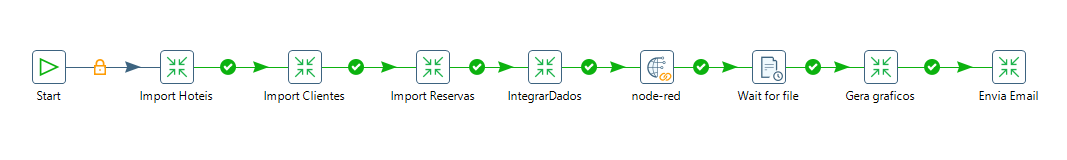
\includegraphics[width=1\textwidth]{images/job.png}
	\caption{Fluxo principal (Job)}
	\label{fig:Job_principal}
\end{figure}
O fluxo principal representa um processo automatizado de integração e processamento de dados. 
O seu objetivo é importar, consolidar, tratar e comunicar informações através de diferentes etapas sequenciais:

\begin{itemize}
	\item \textbf{Import Hoteis} – Importa os dados dos hotéis de um ficheiro XML.
	\item \textbf{Import Clientes} – Importa a informação relativa aos clientes de um ficheiro JSON.
	\item \textbf{Import Reservas} – Importa os dados das reservas efetuadas de um ficheiro CSV.
	\item \textbf{IntegrarDados} – Integra e consolida os dados importados, estabelecendo relações entre hotéis, clientes e reservas.
	\item \textbf{node-red} – Executa um fluxo no Node-RED para gerar gráficos com os dados transformados e gerar tambem ficheiros JSON que serão utilizados de seguida no script \textit{python} para gerar gráficos localmente.
	\item \textbf{Wait for file} – Aguarda a chegada de um ficheiro externo do node-red para gerar novos gráficos.
	\item \textbf{Gera gráficos} – Gera representações gráficas a partir dos dados processados.
	\item \textbf{Envia Email} – Envia um email automático com os gráficos gerados em anexo.
\end{itemize}


Este job representa um pipeline completo de integração de dados, 
desde a importação até à comunicação dos resultados.

\section{Descrição das Transformações}

\subsection{ImportHoteis.ktr}
\begin{figure}[h] 
	\centering 
	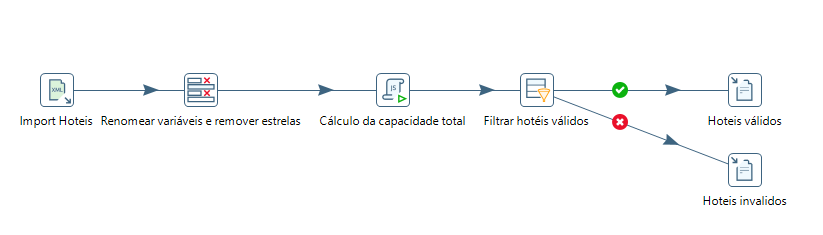
\includegraphics[width=0.9\textwidth]{images/hoteis.png}
	\caption{Transformação dos hotéis}
	\label{fig:transformacao_hoteis}
\end{figure}

\begin{itemize}
	\item \textbf{Import Hoteis} – Importa os dados brutos de hotéis a partir de um ficheiro externo em formato XML.
	\item \textbf{Renomear variáveis e remover estrelas} – Efectua a limpeza e normalização dos dados, renomeando colunas e removendo o campo de classificação por estrelas.
	\item \textbf{Cálculo da capacidade total} – Calcula a capacidade total de cada hotel, no caso multiplica o número de quartos por 2 considerando que cada quarto tem capacidade para duas pessoas.
	\item \textbf{Filtrar hotéis válidos} – Verifica se o número de quartos do hotel é superior a 0.
	\item Os \textbf{hotéis válidos} são exportados para um ficheiro designado \textit{Hotéis válidos}.
	\item Os \textbf{hotéis inválidos} são guardados num ficheiro separado chamado \textit{Hotéis inválidos}.
\end{itemize}

\subsection{ImportClientes.ktr}

\begin{figure}[h] 
	\centering 
	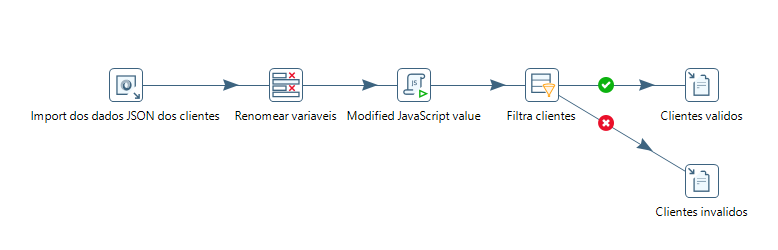
\includegraphics[width=1\textwidth]{images/clientes.png}
	\caption{Transformação dos clientes}
	\label{fig:transformacao_clientes}
\end{figure}


\begin{itemize}
	\item \textbf{Import dos dados JSON dos clientes} – Importa a informação dos clientes a partir de um ficheiro no formato JSON.
	\item \textbf{Renomear variáveis} – Normaliza os nomes das variáveis, tornando-os consistentes e adequados ao modelo de dados interno.
	\item \textbf{Modified JavaScript value} – Verifica se o email do utilizador é válido ou não.
	\item \textbf{Filtra clientes} – Filtra os registos de clientes de acordo com critérios de validade.
	\item Os \textbf{clientes válidos} são exportados para um ficheiro denominado \textit{Clientes válidos}.
	\item Os \textbf{clientes inválidos} são guardados num ficheiro separado chamado \textit{Clientes inválidos}.
\end{itemize}

\newpage

\subsection{ImportReservas.ktr}

\begin{figure}[h] 
	\centering 
	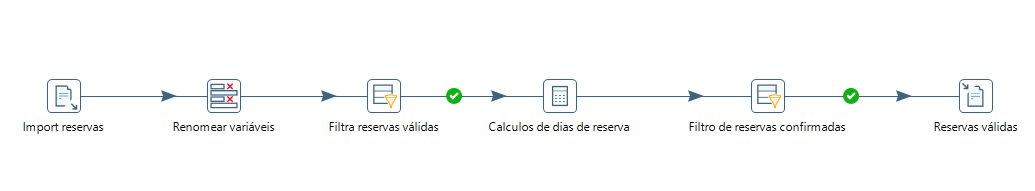
\includegraphics[width=1\textwidth]{images/reservas.png}
	\caption{Transformação das reservas}
	\label{fig:transformacao_reservas}
\end{figure}

\begin{itemize}
	\item \textbf{Importar reservas} – Importa os dados das reservas a partir de um ficheiro csv.
	\item \textbf{Renomear variáveis} – Normaliza os nomes das colunas, tornando-os consistentes e adequados ao processamento interno.
	\item \textbf{Filtrar reservas válidas} – Filtra os registos de reservas com preços superiores a 0.
	\item \textbf{Cálculo de dias de reserva} – Calcula o número de dias de cada reserva com base nas datas de check-in e check-out.
	\item \textbf{Filtrar reservas confirmadas} – Mantém apenas as reservas que estão confirmadas.
	\item \textbf{Reservas válidas} – O resultado final é um conjunto de reservas válidas e confirmadas, pronto para utilização ou exportação.
\end{itemize}
\newpage
\subsection{IntegrarDados.ktr}

\begin{figure}[h] 
	\centering 
	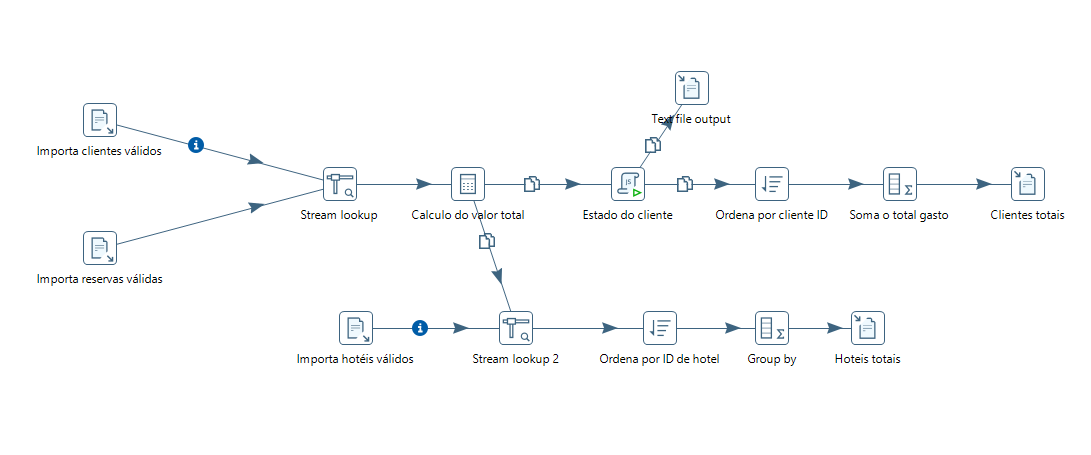
\includegraphics[width=1\textwidth]{images/integrar_dados.png}
	\caption{Transformação das reservas}
	\label{fig:transformacao_integrar_dados}
\end{figure}

Esta transformação tem como objetivo integrar e analisar dados de clientes, reservas e hotéis, de forma a calcular o valor total gasto por cliente e as estatísticas agregadas por hotel.

\begin{itemize}
	\item \textbf{Importa clientes válidos} – Importa os registos de clientes previamente validados.
	\item \textbf{Importa reservas válidas} – Importa as reservas consideradas válidas após o processo de filtragem.
	\item \textbf{Stream lookup} – Junta os dados de clientes e reservas com base no identificador comum, permitindo combinar informação relevante de ambos.
	\item \textbf{Cálculo do valor total} – Calcula o valor total associado a cada reserva, considerando as variáveis necessárias (como número de dias e preço).
	\item \textbf{Importa hotéis válidos} – Importa os dados dos hotéis previamente validados.
	\item \textbf{Stream lookup 2} – Associa as reservas aos respetivos hotéis, enriquecendo os dados com informação do estabelecimento.
	\item \textbf{Estado do cliente} – Verifica se o cliente é válido ou inválido.
	\item \textbf{Ordena por cliente ID} – Organiza os dados por identificador de cliente para facilitar o agrupamento e cálculo posterior.
	\item \textbf{Soma o total gasto} – Calcula o total gasto por cliente, consolidando todas as suas reservas.
	\item \textbf{Clientes totais} – Exporta o resultado agregado por cliente, representando o total gasto.
	\item \textbf{Ordena por ID de hotel} – Ordena os registos por identificador de hotel para o processamento seguinte.
	\item \textbf{Group by} – Soma o valor ganho por cada hotel com as reservas.
	\item \textbf{Hotéis totais} – Gera o resultado final com as estatísticas globais de cada hotel.
	\item \textbf{Text file output} – Exporta os dados das reservas para um ficheiro.
\end{itemize}

\subsection{GeraGraficos.ktr}

\begin{figure}[h] 
	\centering 
	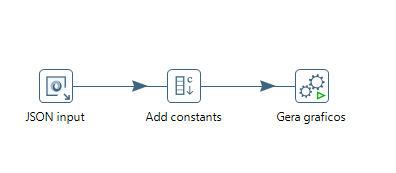
\includegraphics[width=1\textwidth]{images/gera_graficos.png}
	\caption{Transformação de gerar gráficos}
	\label{fig:transformacao_gera_graficos}
\end{figure}

\begin{itemize}
	\item \textbf{JSON input} – Importa os dados dos gráficos gerados pelo node-red.
	\item \textbf{Add constants} – Cria constantes com o valor do comando a ser executado no nó a seguir, neste caso o comando \textit{python}, e o path do ficheiro \textit{.py} a ser executado.
	\item \textbf{Gera graficos} – Executa o script python que cria os gráficos.
\end{itemize}
\newpage
\subsection{EnviaEmail.ktr}

\begin{figure}[h] 
	\centering 
	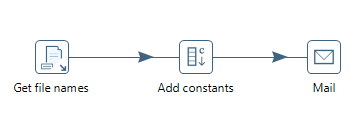
\includegraphics[width=1\textwidth]{images/envia_email.png}
	\caption{Transformação de enviar email}
	\label{fig:transformacao_envia_email}
\end{figure}

\begin{itemize}
	\item \textbf{Get file names} – Importa o nome dos ficheiros com os gráficos em .png.
	\item \textbf{Add constants} – Cria constantes com o que é necessário para enviar o email.
	\item \textbf{Mail} – Envia email com as imagens dos gráficos em anexo.
\end{itemize}
\section{Fluxo node-red}
Foram desenvolvidos dois fluxos distintos na plataforma Node-RED com objetivos complementares.  
O primeiro fluxo tem como finalidade a \textbf{criação de ficheiros com dados aleatórios}, simulando informação de clientes, reservas e hotéis, utilizada posteriormente para análise e visualização.  
O segundo fluxo é responsável pela \textbf{geração de gráficos} a partir desses dados, permitindo representar visualmente as receitas por hotel e o total gasto por cliente.  
Este último fluxo inicia-se através de um pedido HTTP e integra etapas de leitura, conversão, tratamento e exportação dos dados em formato JSON, assegurando a automatização do processo de criação dos gráficos.
\subsection{Fluxo de dados aleatórios}
\begin{figure}[H] 
	\centering 
	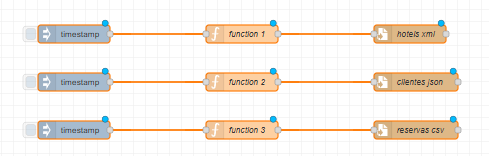
\includegraphics[width=1\textwidth]{images/node-red_ficheiros.png}
	\caption{Fluxo node-red para gerar ficheiros}
	\label{fig:node-red_gerar_ficheiros}
\end{figure}
Neste caso será descrito apenas o fluxo de geração de dados dos \textbf{hotéis}, uma vez que os fluxos relativos aos \textbf{clientes} e às \textbf{reservas} apresentam a mesma estrutura e funcionamento, variando apenas no tipo de dados gerados.  

\begin{itemize}
	\item \textbf{Timestamp} – Inicia o processo de geração de dados de forma manual, permitindo executar o fluxo sempre que necessário.
	\item \textbf{Function 1} – Cria dados aleatórios referentes aos hotéis, simulando atributos como identificadores, nomes, estrelas, país, cidade e número de quartos.
	\item \textbf{Hotels XML} – Exporta os dados gerados para um ficheiro no formato \texttt{XML}, armazenando a informação simulada para utilização posterior nos restantes fluxos.
\end{itemize}
\newpage
\subsection{Fluxo de gerar gráficos}
\begin{figure}[H] 
	\centering 
	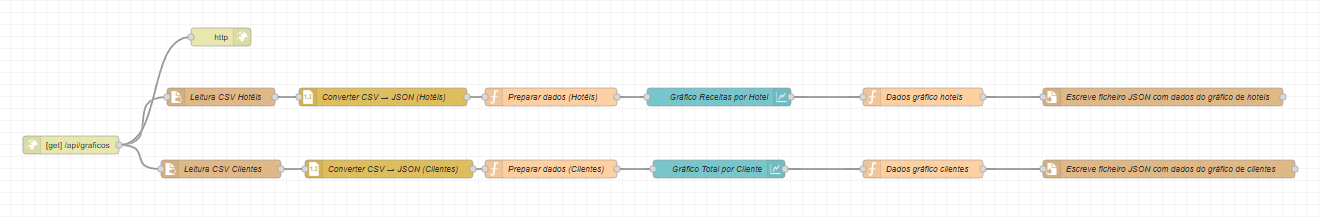
\includegraphics[width=1\textwidth]{images/node-red_graficos.png}
	\caption{Fluxo node-red para gerar graficos}
	\label{fig:node-red_gerar_graficos}
\end{figure}

Neste ponto será apresentado apenas o fluxo correspondente aos \textbf{hotéis}, uma vez que o processo relativo aos \textbf{clientes} é idêntico em estrutura e funcionamento, diferindo apenas nos dados utilizados.  

\begin{itemize}
	\item \textbf{HTTP GET /apigraficos} – Inicia o fluxo quando é feita uma requisição HTTP para o endpoint definido, ativando o processo de geração dos gráficos.
	\item \textbf{Leitura CSV Hotéis} – Lê o ficheiro CSV contendo a informação dos hotéis, incluindo dados relevantes como identificadores e receitas.
	\item \textbf{Converter CSV → JSON (Hotéis)} – Converte os dados do ficheiro CSV para o formato JSON, facilitando o seu tratamento nas etapas seguintes.
	\item \textbf{Preparar dados (Hotéis)} – Processa e organiza os dados dos hotéis, calculando os valores necessários para gerar o gráfico.
	\item \textbf{Gráfico Receitas por Hotel} – Cria o gráfico que representa as receitas obtidas por cada hotel com base nos dados processados.
	\item \textbf{Dados gráfico hotéis} – Extrai e formata os dados do gráfico, preparando-os para serem guardados num ficheiro.
	\item \textbf{Escreve ficheiro JSON com dados do gráfico de hotéis} – Exporta os dados do gráfico para um ficheiro em formato JSON, permitindo o seu uso posterior.
\end{itemize}

\newpage

\section{Configuração de caminhos de ficheiros}

Nos nós de entrada e saída de ficheiros do Node-RED foram definidos \textit{paths} absolutos, o que significa que os ficheiros são lidos e gravados num local específico do computador onde o projeto foi desenvolvido.  

Para garantir o correto funcionamento do programa noutros dispositivos, estes caminhos devem ser alterados de acordo com a estrutura de pastas existente no computador em que o sistema for executado. Por exemplo, atualmente os fluxos utilizam caminhos como:  

\begin{verbatim}
	C:\Users\Diogo Machado\Documents\GitHub\ISI\data\output\hoteis_totais.csv
\end{verbatim}

Este caminho deve ser ajustado para a diretoria correspondente no novo computador, assegurando que o Node-RED consegue aceder corretamente aos ficheiros de entrada e criar os ficheiros de saída.

\section{Conclusão}

O desenvolvimento deste trabalho permitiu compreender de forma prática e integrada o funcionamento dos processos de ETL (\textit{Extract, Transform, Load}) e a sua importância na consolidação de dados provenientes de diferentes fontes. Através da utilização das ferramentas Pentaho Data Integration e Node-RED, foi possível construir um sistema completo, capaz de importar, transformar, integrar e visualizar dados de forma automatizada.

A implementação dos fluxos desenvolvidos demonstrou a relevância da normalização e validação da informação, assegurando a consistência dos resultados obtidos. A criação de ficheiros com dados aleatórios e a posterior geração de gráficos permitiram simular um cenário realista de gestão de reservas hoteleiras, evidenciando a utilidade prática dos processos de integração de dados na análise e apoio à decisão.

Para além dos aspetos técnicos, este projeto contribuiu também para o reforço de competências na configuração e interoperabilidade entre diferentes ferramentas, nomeadamente na comunicação entre o Pentaho e o Node-RED. A atenção aos detalhes, como a definição de \textit{paths} e dependências externas, revelou-se essencial para garantir a portabilidade e o correto funcionamento do sistema em diferentes ambientes.

Em suma, o trabalho cumpriu os objetivos propostos, demonstrando a aplicação eficaz dos conceitos de integração de sistemas de informação e destacando o potencial das ferramentas de ETL e automação na gestão e visualização de dados empresariais.

\section{Repositório Git}

O repositório de GitHub pode se encontrar \href{https://github.com/DiogoMachado04/ISI}{aqui}.

\section{Visualização do video}

Para visualizar o vídeo com a demonstração faça scan do seguinte QR code:

\begin{figure}[h] 
	\centering 
	
\includegraphics[width=0.5\textwidth]{images/qr_code.png}
	\caption{QR code}
	\label{fig:qr_code}
\end{figure}
%----------------------------------------------------------------------------------------
%	BIBLIOGRAPHY

%----------------------------------------------------------------------------------------

\end{document}